\documentclass[11pt,a4paper]{article}
\usepackage{fontspec}
\setmainfont{TeX Gyre Pagella}
\newfontfamily\headfont{Inter}[UprightFont=*-ExtraBold,BoldFont=*-ExtraBold,Extension=.otf,Path=/usr/share/fonts/opentype/inter/]
\usepackage[a4paper,margin=2.3cm]{geometry}
\usepackage{graphicx,booktabs,float,caption,array,xcolor,longtable}
\usepackage{xurl}
\usepackage[hidelinks]{hyperref}
\usepackage{titlesec}
\usepackage[round]{natbib}
\usepackage{setspace}
\setstretch{1.05}
\renewcommand{\topfraction}{0.9}
\renewcommand{\bottomfraction}{0.8}
\renewcommand{\textfraction}{0.1}
\renewcommand{\floatpagefraction}{0.75}
\setlength{\parindent}{0pt}
\setlength{\parskip}{0.55em}
\titleformat{\section}{\headfont\Large}{\thesection}{0.8em}{}
\titleformat{\subsection}{\headfont\large}{\thesubsection}{0.8em}{}
\captionsetup{font=small,labelfont=bf}
\urlstyle{same}
\hypersetup{pdftitle={Towns with an asteroid},pdfauthor={Tristan Hotham}}

\begin{document}
\begin{center}
{\Large\bfseries Towns with an Asteroid\par}
\vspace{0.4em}
{\large The places on Earth that minor planets are named after,\\and the observatories that named them\par}
\vspace{1.2em}
{\large Tristan Hotham\par}
\vspace{0.3em}
{\small Independent researcher\\
ORCID: 0000-0003-4931-9349\\
DOI: https://doi.org/10.5281/zenodo.24052725\par}
\vspace{0.8em}
2026
\end{center}

\begin{quote}
\small
\begin{center}\textbf{Abstract}\end{center}
Discoverers of asteroids propose their names, and many choose places. Using Wikidata's "named after" statements for 11,268 asteroids, I identify 2,206 namings of places with coordinates, on 2,193 asteroids (19.3\% of all namings; 65.4\% honour people) and link each place to the site where its asteroid was discovered. Towns, cities and villages make up 52.1\% of the places. Japan has the most (421); per head, Finland (11.8 per million people), the Czech Republic (9.8) and Sweden (8.1) lead. The median distance from discovery site to named place is 508 km and 27.1\% of places lie within 100 km. Naming geography follows the astronomer: only 3.6\% of the places named from La Silla in Chile are Chilean, while Kle\v{t} Observatory named 98 places, 80.6\% of them Czech and 50.0\% within 100 km, and 92.5\% of Japanese places were named from Japanese observatories. I describe the data, its incompleteness and the classification, and publish the linked tables and an interactive map.

\textbf{Keywords:} minor planets; asteroids; nomenclature; toponymy; commemoration; amateur astronomy; Wikidata; open data; mapping
\end{quote}

\section{Introduction}
Once an asteroid's orbit is secure it receives a number, and its discoverer may propose a name, which the International Astronomical Union's Working Group Small Bodies Nomenclature considers and publishes \citep{mpc,wgsbn}. The result is a large, informal archive of what astronomers chose to remember: colleagues and family, scientists and artists, and places. Many place names are personal. An observatory names its own town and the villages around it; an astronomer abroad names the town where they grew up.

This paper maps that naming geography with open data. Wikidata \citep{wikidata} records, for many asteroids, what they are named after, where they were discovered and by whom. Joining the two gives each named place a line to the observatory that found its asteroid. I ask which places have an asteroid, which countries have most, who named them, and how close to home.

\section{Data}
A single query of Wikidata through QLever \citep{qlever} returned every item that is an asteroid (an instance of asteroid or of a subclass) with a "named after" (P138) statement, with its minor planet number, discoverer (P61), discovery site (P65) and its coordinates and country, discovery date, and the namesake's type, coordinates and country. The query returned 22,704 rows, one per discoverer and type, describing 11,268 asteroids and 11,418 asteroid and namesake pairs (``namings''); 133 asteroids have more than one namesake. Wikidata is released under CC0. Natural Earth \citep{naturalearth} gives modern countries and their population estimates.

Wikidata does not record the namesake of every named minor planet, and I have not compared these records with the Minor Planet Center's complete list of names. The data are therefore the subset of named minor planets that Wikidata links to a namesake, not all named minor planets, and its coverage may differ by country and period.

\section{Methods}
\subsection{Places and kinds}
A namesake is a person if Wikidata says it is human (Q5); otherwise it is a place if it has coordinates and is not mythical or fictional. Namesakes that have coordinates but are not places are also ``other'': any whose Wikidata types include a language, a taxon, a ship, a battle or other event, a television programme, a people or ethnic group, a dynasty or a troupe; bodies whose types are all organisational (an agency, society, ministry, survey or league with no site of its own); and two cases found by hand (a star party and a government department typed as an observatory and a region). I read the whole resulting list of places by eye. Everything else (gods, works, organisations without coordinates) is ``other'' too. Places were sorted into kinds by keyword rules applied, in order, to all of their Wikidata types: rivers, lakes and seas; towns, cities and villages; countries (exact types such as ``sovereign state'' or ``historical country''); observatories, universities and other institutions; mountains, islands and other natural features; and regions, provinces and counties. A small remainder is ``other places''.

\subsection{Countries, distances and home}
Each place and each discovery site is given the modern country Wikidata records for it (P17) when that names exactly one modern country and the point lies within about 30 km of that country's Natural Earth outline, which settles border towns such as Passau, Konstanz, Gorizia and Tornio; otherwise (no country, several, or only a historical state) it is placed in a Natural Earth country by its coordinates. Continents are assigned to no country. Crimea, where Natural Earth's default view places it in Russia, is counted as Ukraine. Per head rates use Natural Earth's population estimates (mostly for 2019) and are reported for countries of at least a million people with five or more place namings. Populations are Natural Earth country figures, so Hong Kong and other territories count separately. Distances are great circle distances between the discovery site and the place's single point, so they are rough for regions, rivers and countries. A place is ``home'' if it is in the same country as the discovery site.

\section{Results}
\subsection{What is named}
Of the 11,418 namings, 7,463 (65.4\%) honour people, 2,206 (19.3\%) places with coordinates and 1,749 (15.3\%) other things (Figure~\ref{fig:kinds}). The 2,206 place namings cover 2,175 distinct places: 1,150 namings of towns, cities and villages, 309 of institutions, 280 of natural features, 191 of regions, 140 of rivers and lakes and 82 of countries. Figure~\ref{fig:world} maps them all.

\begin{figure}[tbp]\centering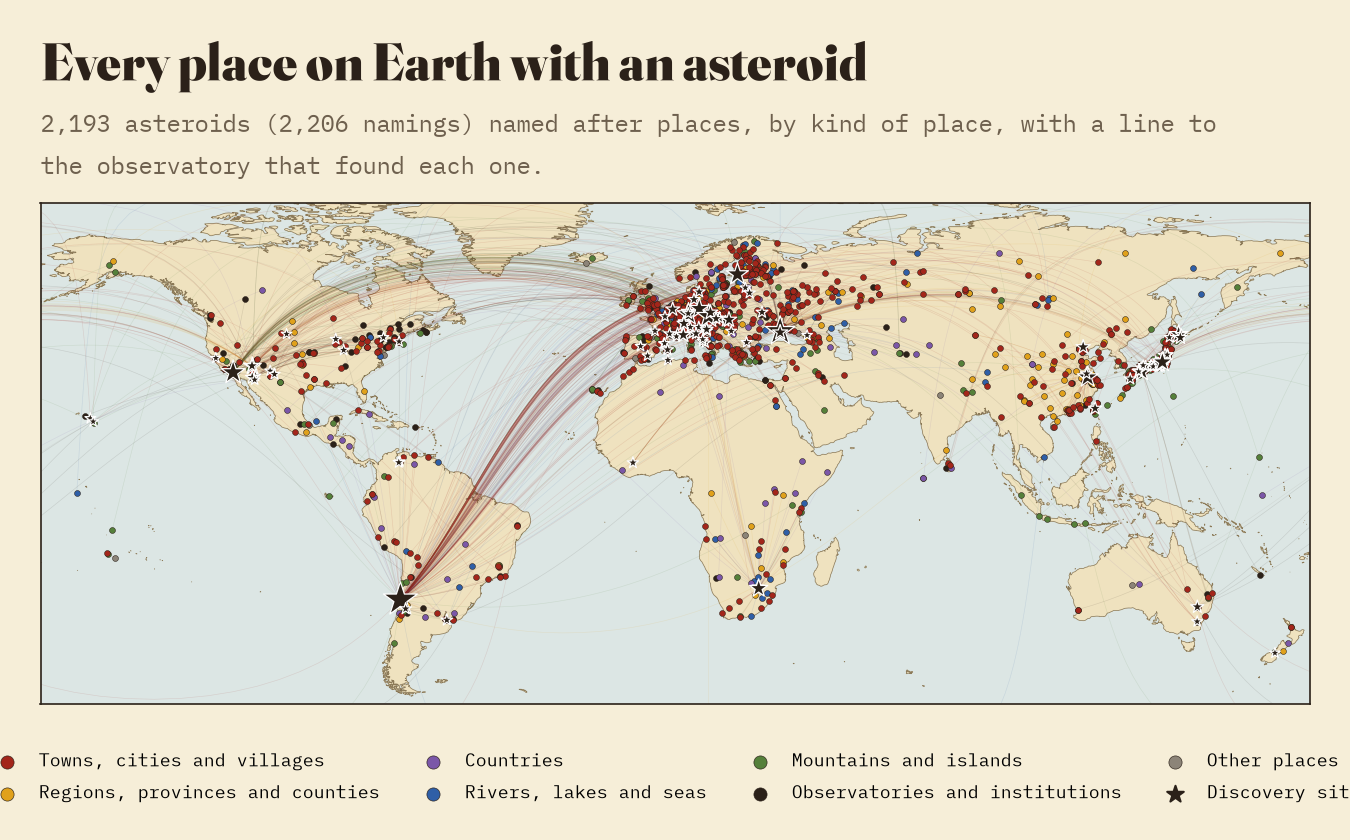
\includegraphics[width=\textwidth]{f_world.png}
\caption{Every place with an asteroid in Wikidata, by kind, with great circle lines to the discovery sites.}\label{fig:world}\end{figure}
\begin{figure}[tbp]\centering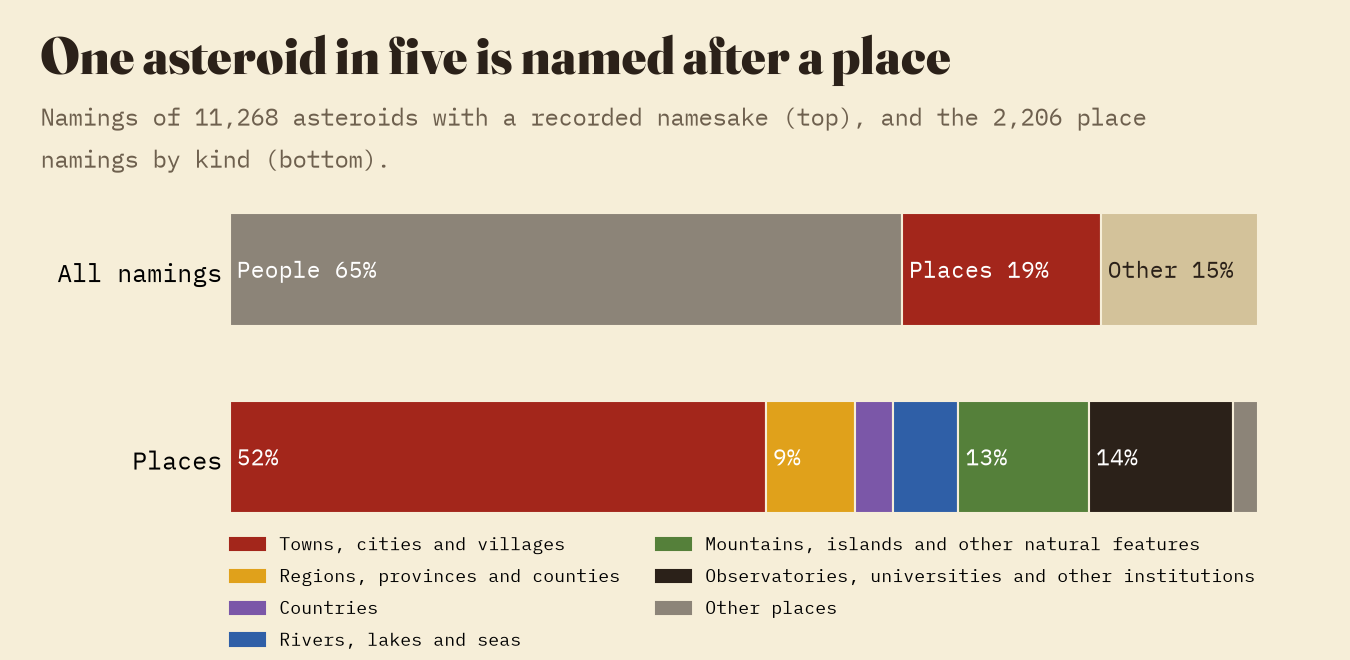
\includegraphics[width=\textwidth]{f_kinds.png}
\caption{People, places and other namesakes (top) and the kinds of place (bottom).}\label{fig:kinds}\end{figure}

\subsection{Countries}
Places in 111 modern countries have an asteroid. Japan leads with 421 (19.1\%), followed by Germany (153), Russia (137), Italy (135) and the United States (130) (Table~\ref{tab:cty}, Figure~\ref{fig:cty}). Per head, Finland, the Czech Republic and Sweden lead, each with long traditions of asteroid discovery.

\begin{table}[tbp]\centering\small\caption{The fifteen countries with the most place namings.}\label{tab:cty}\begin{tabular}{lrrr}\toprule Country & Places & Share (\%) & Per million\\\midrule
Japan & 421 & 19.1 & 3.33\\
Germany & 153 & 6.9 & 1.84\\
Russia & 137 & 6.2 & 0.95\\
Italy & 135 & 6.1 & 2.24\\
United States & 130 & 5.9 & 0.40\\
China & 120 & 5.4 & 0.09\\
France & 106 & 4.8 & 1.58\\
Czech Republic & 104 & 4.7 & 9.75\\
Sweden & 83 & 3.8 & 8.07\\
Finland & 65 & 3.0 & 11.77\\
Ukraine & 64 & 2.9 & 1.44\\
Spain & 49 & 2.2 & 1.04\\
Belgium & 43 & 1.9 & 3.74\\
Switzerland & 32 & 1.4 & 3.73\\
Hungary & 32 & 1.4 & 3.28\\
\bottomrule\end{tabular}\end{table}

\begin{figure}[tbp]\centering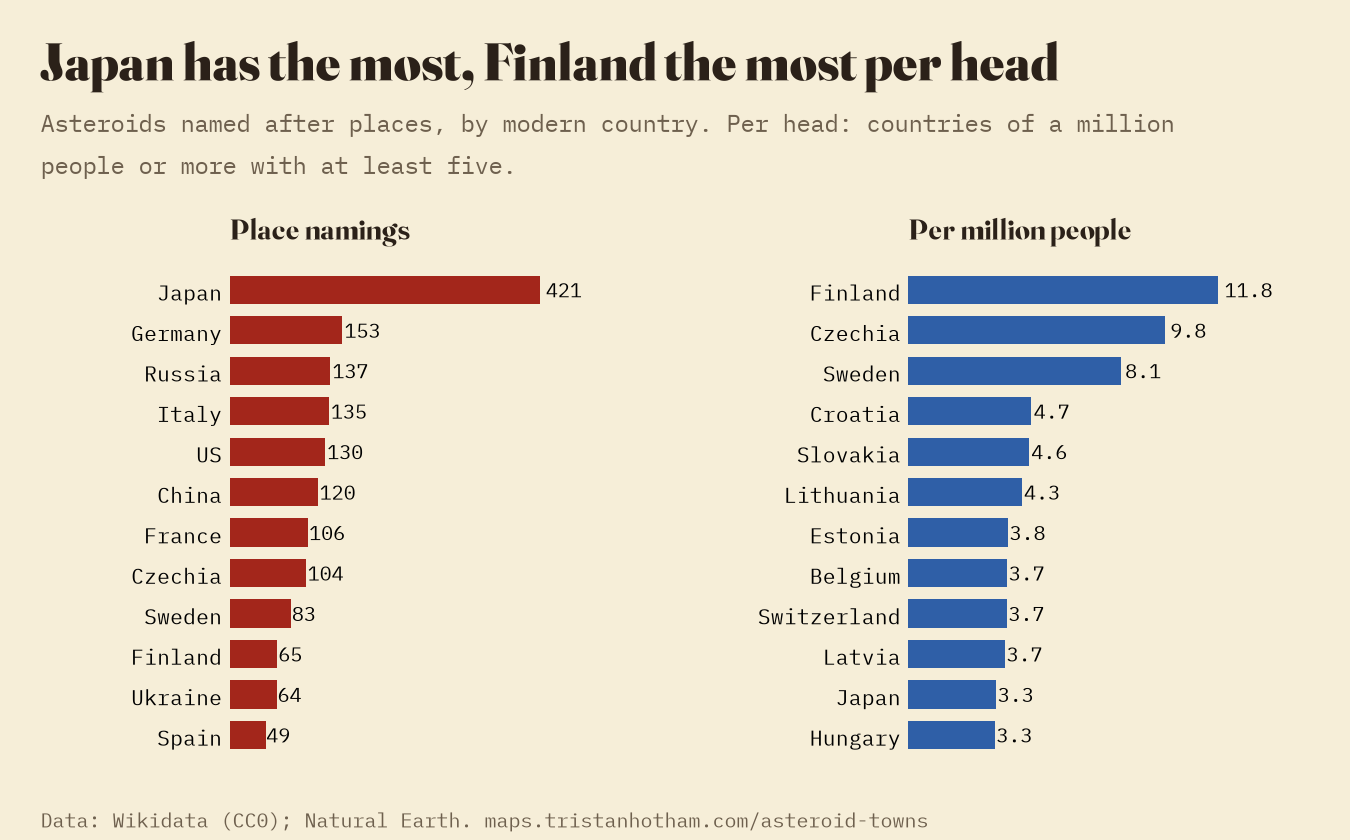
\includegraphics[width=\textwidth]{f_countries.png}
\caption{Place namings by country, in total and per million people.}\label{fig:cty}\end{figure}

\subsection{Who named them}
The 237 discovery sites are led by La Silla (224 place namings), the Crimean Astrophysical Observatory (164) and Palomar (99) (Table~\ref{tab:obs}, Figure~\ref{fig:obs}). Large observatories host visiting astronomers, and their names travel with them: 3.6\% of La Silla's places are in Chile. The Belgian astronomer Eric Elst, the most prolific namer of places in the data (167), worked at La Silla and named 36 places in France and 16 in Belgium; the Uppsala survey at La Silla named Swedish places, so that none of Sweden's 83 places was named from Sweden. Finland is the opposite: all 65 of its places were named from Finnish sites, most by Yrj\"o V\"ais\"al\"a's observatory at Turku. Purple Mountain Observatory named Chinese places almost exclusively (98.6\%).

\begin{table}[tbp]\centering\footnotesize\caption{The fifteen discovery sites with the most place namings: share in the site's own country, median distance and share within 100 km.}\label{tab:obs}\begin{tabular}{llrrrr}\toprule Site & Country & Places & Own (\%) & Median km & $<$100 km (\%)\\\midrule
La Silla Observatory & Chile & 224 & 3.6 & 11,631 & 1.8\\
Crimean Astrophysical Observatory & Ukraine (Crimea) & 164 & 25.6 & 1,251 & 9.8\\
Palomar Observatory & United States & 99 & 21.2 & 9,177 & 1.0\\
Kleť Observatory & Czech Republic & 98 & 80.6 & 101 & 50.0\\
Heidelberg-Königstuhl State Observatory & Germany & 86 & 27.9 & 795 & 14.0\\
Iso-Heikkilä Observatory & Finland & 81 & 79.0 & 364 & 13.6\\
Purple Mountain Observatory & China & 72 & 98.6 & 993 & 5.6\\
Karl Schwarzschild Observatory & Germany & 63 & 74.6 & 285 & 25.4\\
Ōizumi Observatory & Japan & 63 & 96.8 & 120 & 41.3\\
Kitami Observatory & Japan & 51 & 96.1 & 245 & 27.5\\
Union Observatory & South Africa & 49 & 34.7 & 1,471 & 2.0\\
Geisei observatory & Japan & 48 & 85.4 & 117 & 45.8\\
Anderson Mesa Station & United States & 44 & 22.7 & 9,089 & 4.5\\
Piszkéstető Station & Hungary & 30 & 93.3 & 174 & 36.7\\
Simeiz Observatory & Ukraine (Crimea) & 28 & 32.1 & 976 & 21.4\\
\bottomrule\end{tabular}\end{table}

\begin{figure}[tbp]\centering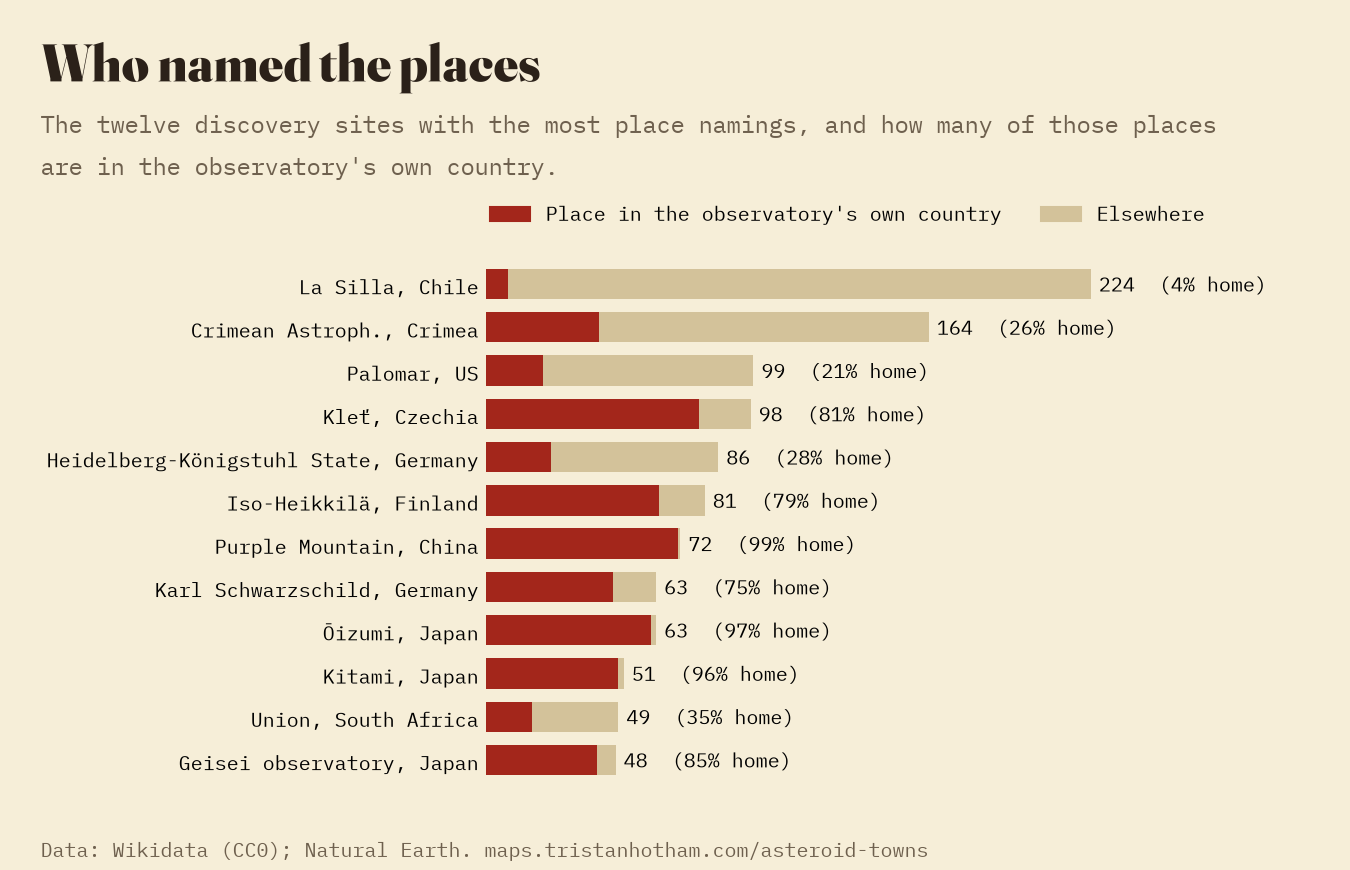
\includegraphics[width=\textwidth]{f_observatories.png}
\caption{The twelve discovery sites with the most place namings, and the share in their own country.}\label{fig:obs}\end{figure}

\subsection{Close to home}
The distribution of distances is wide (Figure~\ref{fig:dist}). The median is 508 km; 27.1\% of places lie within 100 km of the discovery site, and 204 within 10 km, many of them observatories named after themselves (26 of the 82 asteroids named after observatories or telescopes were found there). 58.5\% of places are in the discovery site's country. The most local namers are small observatories with a resident team (Figure~\ref{fig:home}): Kle\v{t} in South Bohemia (50.0\% within 100 km), and Japanese sites such as Nanyo (68.2\%) and Geisei (45.8\%). Of the places in Japan, 92.5\% were named from Japanese sites and 46.1\% from within 100 km; for the Czech Republic the figures are 90.4\% and 54.8\%, and for Italy 49.2\% and 37.7\%.

\begin{figure}[tbp]\centering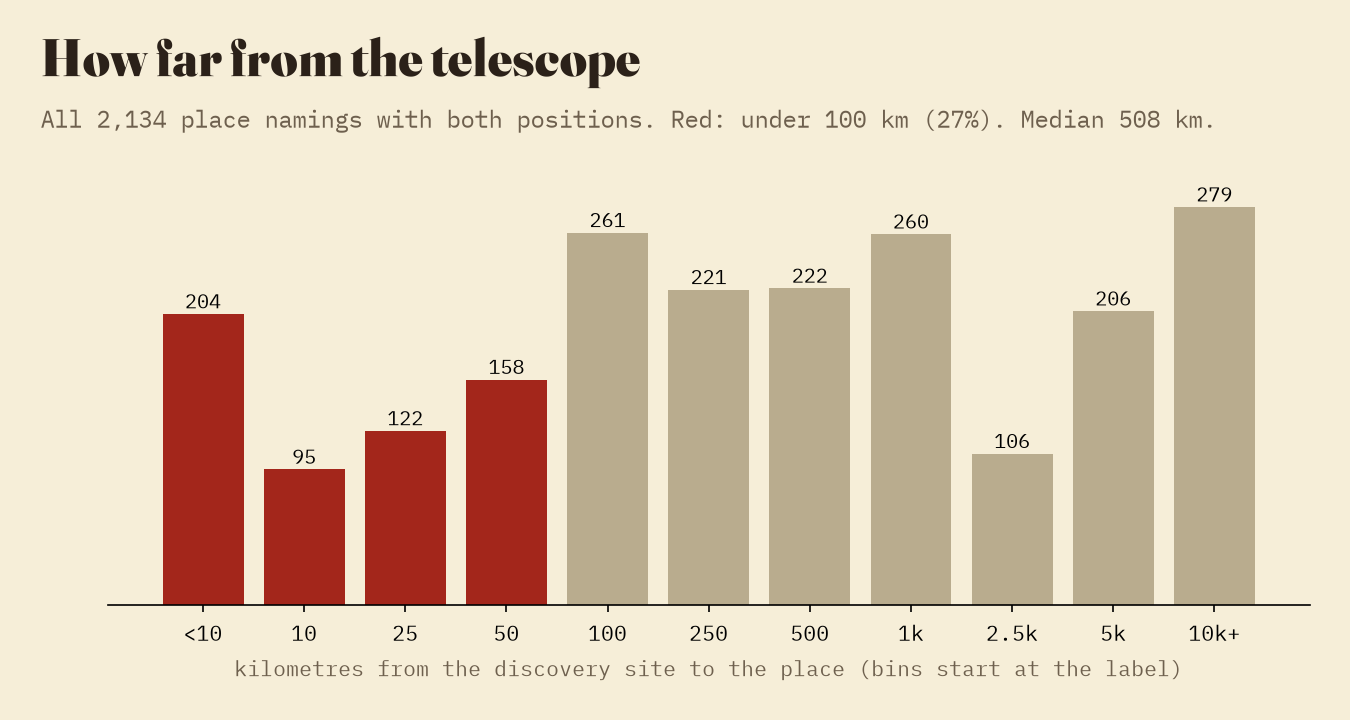
\includegraphics[width=\textwidth]{f_distance.png}
\caption{Distance from discovery site to named place.}\label{fig:dist}\end{figure}
\begin{figure}[tbp]\centering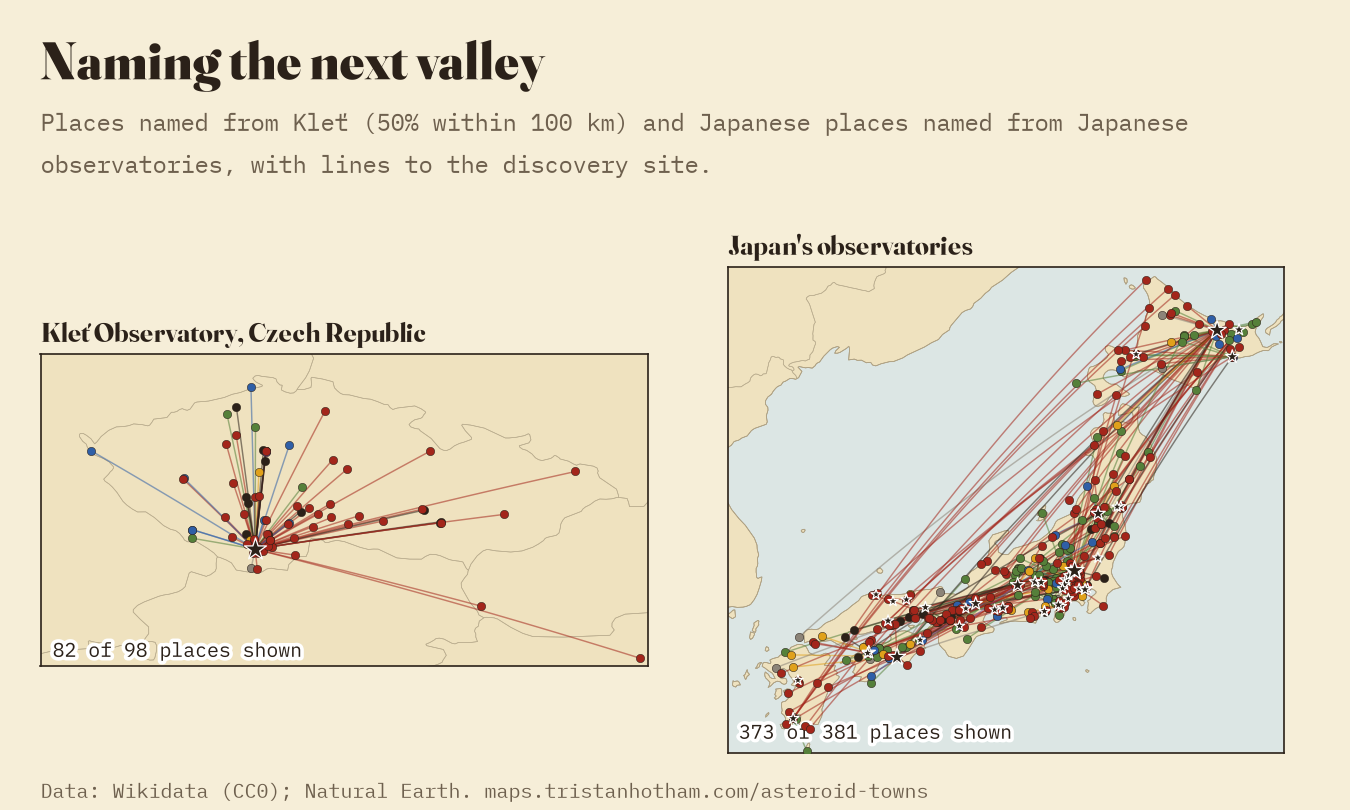
\includegraphics[width=\textwidth]{f_home.png}
\caption{Local naming: places named from Kle\v{t} Observatory, and places in Japan named from Japanese observatories.}\label{fig:home}\end{figure}

\subsection{The United Kingdom}
26 asteroids are named after places in the United Kingdom (16 towns and cities). Nearly all were discovered abroad. The exceptions are an amateur observatory at Church Stretton, Shropshire, which found the asteroids named after Church Stretton and Shropshire (Salopia), and one at Stakenbridge, which found Old Joe, named after the University of Birmingham's clock tower (Table~\ref{tab:uk}).

{\footnotesize\begin{longtable}{p{3.4cm}p{4.2cm}p{4.6cm}rr}\caption{Asteroids named after places in the United Kingdom.}\label{tab:uk}\\\toprule Asteroid & Place & Discovery site & Year & km\\\midrule\endfirsthead\toprule Asteroid & Place & Discovery site & Year & km\\\midrule\endhead
758 Mancunia & Manchester & Union Observatory & 1912 & 9,328\\
1071 Brita & Great Britain & Simeiz Observatory & 1924 & 2,811\\
1244 Deira & Kingdom of Deira & Union Observatory & 1932 & 9,329\\
2531 Cambridge & Cambridge & Anderson Mesa Station & 1980 & 8,270\\
2830 Greenwich & Royal Observatory & Anderson Mesa Station & 1980 & 8,313\\
3009 Coventry & Coventry & Crimean Astrophysical Observatory & 1973 & 2,719\\
3858 Dorchester & Dorchester & Brorfelde Observatory & 1986 & 1,084\\
4206 Verulamium & Verulamium & La Silla Observatory & 1986 & 11,306\\
5677 Aberdonia & University of Aberdeen & Lowell Observatory & 1987 & 7,824\\
5805 Glasgow & Glasgow & Lowell Observatory & 1985 & 7,798\\
6939 Lestone & Leighton Buzzard & Mount Wilson Observatory & 1952 & 8,672\\
7603 Salopia & Shropshire & Church Stretton & 1995 & 11\\
8283 Edinburgh & Edinburgh & Siding Spring Observatory & 1991 & 16,524\\
8380 Tooting & Tooting & Palomar Observatory & 1992 & 8,751\\
8837 London & London & La Silla Observatory & 1989 & 11,305\\
8849 Brighton & Brighton & La Silla Observatory & 1990 & 11,263\\
9325 Stonehenge & Stonehenge & La Silla Observatory & 1989 & 11,186\\
9767 Midsomer Norton & Midsomer Norton & Siding Spring Observatory & 1992 & 16,796\\
10501 Ardmacha & Armagh & Palomar Observatory & 1987 & 8,209\\
10502 Armaghobs & Armagh Observatory & Palomar Observatory & 1987 & 8,209\\
10515 Old Joe & Joseph Chamberlain Memorial Clock Tower & Stakenbridge observatory & 1989 & 16\\
11626 Church Stretton & Church Stretton & Church Stretton & 1996 & 0\\
28220 York & York & Kleť Observatory & 1998 & 1,203\\
69423 Openuni & The Open University & Astronomical Observatory of Farra d'Isonzo & 1996 & 1,238\\
100604 Lundy & Lundy & Royal Observatory of Belgium & 1997 & 633\\
129092 Snowdonia & Snowdon & Haleakalā Observatory & 2004 & 11,384\\
\bottomrule\end{longtable}}

\section{Limitations}
First, coverage: Wikidata records the namesake of only part of the named minor planets, and the share may vary by period, country and discoverer. Second, the observatory is the place of discovery, not certainly the place of naming, and names are sometimes proposed by people other than the discoverer. Third, kinds come from keyword rules on Wikidata's types and are approximate. Fourth, regions, rivers and countries are single points, so their distances are rough. Fifth, modern borders are applied throughout, and Crimea is assigned to Ukraine.

\section{Conclusion}
About one asteroid in five with a recorded namesake honours a place. Japan's dense network of amateur and municipal observatories has put more of its towns in the sky than any other country, and small European observatories such as Kle\v{t} have named their own valleys. Large international observatories spread names around the world, carried by visiting astronomers. Linking open data on asteroids and places makes this naming geography visible and checkable.

\section*{Data and code availability}
The interactive map is at \url{https://maps.tristanhotham.com/asteroid-towns/}. Data and code are at \url{https://github.com/Tristan-Hotham/asteroid-towns} and archived with this paper at https://doi.org/10.5281/zenodo.24052725. Derived data and text are released under CC BY 4.0 (the Wikidata source is CC0); code under the MIT licence.

\section*{AI statement}
I wrote the text, with drafting and editing assistance from Claude (Anthropic), which also helped prepare the analysis code. I reviewed and checked all text and results.

\begin{thebibliography}{9}
\bibitem[Bast and Buchhold(2017)]{qlever} Bast, H. and Buchhold, B. (2017) QLever: a query engine for efficient SPARQL+Text search. In \textit{Proceedings of the 2017 ACM Conference on Information and Knowledge Management (CIKM)}, 647 to 656.
\bibitem[Minor Planet Center(2026)]{mpc} Minor Planet Center (2026) How are asteroids named? \url{https://docs.minorplanetcenter.net/mpc-ops-docs/designations/how-asteroids-are-named/}
\bibitem[Natural Earth(2026)]{naturalearth} Natural Earth (2026) Admin 0 countries, 1:10m. Public domain. \url{https://www.naturalearthdata.com/}
\bibitem[Vrande\v{c}i\'c and Kr\"otzsch(2014)]{wikidata} Vrande\v{c}i\'c, D. and Kr\"otzsch, M. (2014) Wikidata: a free collaborative knowledgebase. \textit{Communications of the ACM} 57(10), 78 to 85.
\bibitem[WGSBN(2026)]{wgsbn} IAU Working Group Small Bodies Nomenclature (2026) WGSBN. \url{https://www.wgsbn-iau.org/}
\end{thebibliography}
\end{document}
